\section{Appendix}
\begin{algorithm}
	\caption{Overall Optimization Algorithm}
	\label{alg1}
	\begin{algorithmic}
		\renewcommand{\algorithmicrequire}{ \textbf{Inputs:}}
		\REQUIRE 
		\STATE Table \ref{tab:common input}: Common input parameters
            \STATE $b^t_u$: Default bandwidth of PoP $u$ in time slot $t$. It refers to the bandwidth of PoP $u$ before scheduling considering all flows egressing via their respective default {\egress} 
            \STATE $d_t$: Egress demand from the WAN in time slot $t$
		
		\renewcommand{\algorithmicensure}{ \textbf{Outputs:}}
		\ENSURE 
            
            \STATE $b^t_{(u,v)}$: Bandwidth of backbone link from PoP $u$ to PoP $v$ in time slot $t$
            \STATE $p_i$: Estimated 95th-percentile billable bandwidth of {\egress} $l_i$
            \STATE $k_{i}^t$: Whether {\egress} $l_i$ bursts in time slot $t$. 
            \STATE $y_i^t$: Maximal available bandwidth of {\egress} $l_i$ in time slot $t$. When $k_{i}^t$ equals 1, $y_i^t$ takes the value of $p_i$; conversely, when $k_{i}^t$ equals 0, $y_i^t$ assumes the value of $C_i$
		
		\renewcommand{\algorithmicensure}{ \textbf{Minimize:}}
		\ENSURE
		$\sum_{l_i \in L} c_i p_i$

		\renewcommand{\algorithmicensure}{ \textbf{Subject to:}}
		\ENSURE
     \begin{subequations}
        \begin{align}
            & \forall l_i \in L : \sum_{t \in J} k_{i}^t=\frac{n}{20}  \label{eq:11} \\
            & \forall l_i \in L : ub_i \leq p_i \label{eq:12} \\
            & \forall(u, v)\in E,\forall t \in J : b_{(u, v)}^t \leq C_{(u, v)} \label{eq:13} \\
            & \forall t \in J : d_t \leq \sum_{l_i \in L} y_i^t  \label{eq:14} \\
            & \forall u \in V_a, \forall t \in J  : \sum_{(v, u) \in E_u^D} b_{(v, u)}^t-\sum_{(u, v) \in E_u^S} b_{(u, v)}^t + b_u^t \leq \sum_{l_i \in L_u} y_i^t   \label{eq:15} \\
            & \forall u \in V_a, \forall t \in J  : \sum_{(u, v) \in E_u^D} b_{(u, v)}^t-\sum_{(u, v) \in E_u^S} b_{(u, v)}^t + b_u^t \geq 0   \label{eq:16}  \\
            & \forall u \in V_p,\forall t \in J : \sum_{(v, u) \in E_u^D} b_{(v, u)}^t=\sum_{(u, v) \in E_u^S} b_{(u, v)}^t   \label{eq:17}  \\
            & \forall t \in J, \forall l_i \in L : y_i^t \leq p_i+M k_{i}^t \label{eq:18} \\
            & \forall t \in J, \forall l_i \in L : y_i^t \geq p_i-M k_{i}^t \label{eq:19} \\
            & \forall t \in J, \forall l_i \in L : y_i^t \leq C_i+M\left(1-k_{i}^t\right)  \label{eq:110}  \\
            & \forall t \in J, \forall l_i \in L : y_i^t \geq C_i-M\left(1-k_{i}^t\right) \label{eq:111}
        \end{align}
    \end{subequations}
	\end{algorithmic}
\end{algorithm}



\begin{algorithm}
	\caption{Time Slot Optimization Algorithm}
	\label{alg3}
	\begin{algorithmic}
		\renewcommand{\algorithmicrequire}{ \textbf{Inputs:}}
		\REQUIRE 
		\STATE Table \ref{tab:common input}: Common input parameters
            \STATE $b^t_u$: Default bandwidth of PoP $u$ in time slot $t$. It refers to the bandwidth of PoP $u$ before scheduling considering all flows egressing via their respective default {\egress} 
            \STATE $t$: Current time slot
            \STATE $F^t=\{f^t\}$: Set of flows in current time slot
            
            
		
		\renewcommand{\algorithmicensure}{ \textbf{Outputs:}}
		\ENSURE 
            
            \STATE $b^t_{(u,v)}$: Bandwidth of backbone link from PoP $u$ to PoP $v$ in time slot $t$
            \STATE $p_i^t$: Estimated $95^{th}$ percentile billable bandwidth of {\egress} $i$
            \STATE $k_{i}^t$: Whether {\egress} $i$ bursts in time slot $t$ 
            \STATE $y_i^t$: Maximal available bandwidth of {\egress} $i$ in time slot $t$
            \STATE $x_{i}^{f^{t}}$: Whether $f^t$ egress via {\egress} $i$  in time slot $t$ 
            \STATE $x_{(u,v))}^{f^{t}}$: Whether $f^t$ go through backbone link $(u,v)$  in time slot $t$ 
		
		\renewcommand{\algorithmicensure}{ \textbf{Minimize:}}
		\ENSURE
		$$\sum_{l_i \in L} c_i \cdot p_i^t+\sum_{f^t \in F_s} w_1\left(V_f\right) x_i^{f^t}          \cdot perf(i, f^t) +w_2 \sum_{l_i \in L} y_i $$

		\renewcommand{\algorithmicensure}{ \textbf{Subject to:}}
		\ENSURE
            $$\begin{array}{ll}
            \forall l_i \in L : &p_i^t \geq p_i^{t-1} \\
            \forall f^{t} \in F^{t} : &\sum_{l_i \in L_f^{t}} x_i^{f^{t}}=1 \\
            \forall l_i \in L : &\sum_{f^{t} \in F^{t}} V_f x_i^{f^{t}} \leq y_i \\
            \forall(u, v) \in E  : &\sum_{f^{t} \in F^{t}} V_f x_{(u, v)}^{f^{t}} \leq C_{(u, v)} \\
            \forall f^{t}, \forall u \text { where } S(f^{t})=u : &\sum_{f^{t} \in F^{t}} x_{(u, v)}^{f^{t}}+\sum_{l_i \in L_u} x_i^{f^{t}}=1 \\
            \forall f^{t}, \forall u \text { where } S(f^{t}) \neq u  : &\sum_{f^{t} \in F^{t}} x_{(u, v)}^{f^{t}}+\sum_{l_i \in L_u} x_i^{f^{t}} \\& =\sum_{f^{t} \in F^{t}} x_{(v, u)}^{f^{t}} \\
            \forall u \in V_a : &\sum_{f^{t} \in F^{t}} \sum_{(v, u) \in E_u^D} V_f x_{(v, u)}^{f^{t}} \\&-\sum_{f^{t} \in F^{t}} \sum_{(u, v) \in E_u^S} V_f x_{(u, v)}^{f^{t}} \\& +b_u^t \leq \sum_{l_i \in L_u} y_i \\
            \forall u \in V_a : &\sum_{f^{t} \in F^{t}} \sum_{(v, u) \in E_u^D} V_f x_{(v, u)}^{f^{t}} \\&-\sum_{f^{t} \in F^{t}} \sum_{(u, v) \in E_u^S} V_f x_{(u, v)}^{f^{t}} \\& +b_u^t \geq 0 \\
            \forall u \in V_p : &\sum_{f^{t} \in F^{t}} \sum_{(v, u) \in E_u^D} V_f x_{(v, u)}^{f^{t}} \\& =\sum_{f^{t} \in F^{t}} \sum_{(u, v) \in E_u^S} V_f x_{(u, v)}^{f^{t}} \\
            \forall l_i \text { without free slots } : &y_i=p_i^t \\
            \forall l_i \text { with free slots } : &y_i \leq p_i^t+M k_i^t \\
            \forall l_i \text { with free slots } : &y_i \geq p_i^t-M k_i^t \\
            \forall l_i \text { with free slots } : &y_i \leq C_i+M\left(1-k_i^t\right) \\
            \forall l_i \text { with free slots } : &y_i \geq C_i-M\left(1-k_i^t\right) \\
            \end{array}$$
	\end{algorithmic}
\end{algorithm}





\begin{algorithm}
	\caption{{\EGRESS} Burst Decision Algorithm}
	\label{alg4}
	\begin{algorithmic}
		\renewcommand{\algorithmicrequire}{ \textbf{Inputs:}}
		\REQUIRE 
		\STATE Table \ref{tab:common input}: Common input parameters
        \STATE $b^t_u$: Default bandwidth of PoP $u$ in time slot $t$. It refers to the bandwidth of PoP $u$ before scheduling considering all flows egressing via their respective default {\egress}
        \STATE $t$: Current time slot
            
		
		\renewcommand{\algorithmicensure}{ \textbf{Outputs:}}
		\ENSURE 
            
            \STATE $b^t_{(u,v)}$: Bandwidth of backbone link from PoP $u$ to PoP $v$ in time slot $t$
            \STATE $k_{i}^t$: Whether {\egress} $i$ bursts in time slot $t$
		
		\renewcommand{\algorithmicensure}{ \textbf{Minimize:}}
		\ENSURE
		$$\sum_{l_i \in L} y_i $$

		\renewcommand{\algorithmicensure}{ \textbf{Subject to:}}
		\ENSURE
            $$\begin{array}{ll}
             \forall l_i \text{ without free slots} : & y_i=p_i\\
             \forall l_i \text{ with free slots} :&y_i=p_i(1-k_i)+C_ik_i\\
            & \sum_{u\in V} b_u^t\le \sum_{l_i \in L} y_i \\
             \forall(u,v) \in E :&b_{(u,v)}^t \le C_{(u,v)}\\
             \forall u \in V : & \sum_{(u,v)\in E_u^D} b_{(u,v)}^t - \sum_{(u,v)\in E_u^S} b_{(u,v)}^t\\& + b_u^t\le \sum_{l_i\in L_u} y_i\\
             \forall u \in V :& \sum_{(u,v)\in E_u^D} b_{(u,v)}^t - \sum_{(u,v)\in E_u^S} b_{(u,v)}^t\\ & + b_u^t \ge 0\\
            
            \end{array}$$
	\end{algorithmic}
\end{algorithm}


\begin{figure}
	\centering
	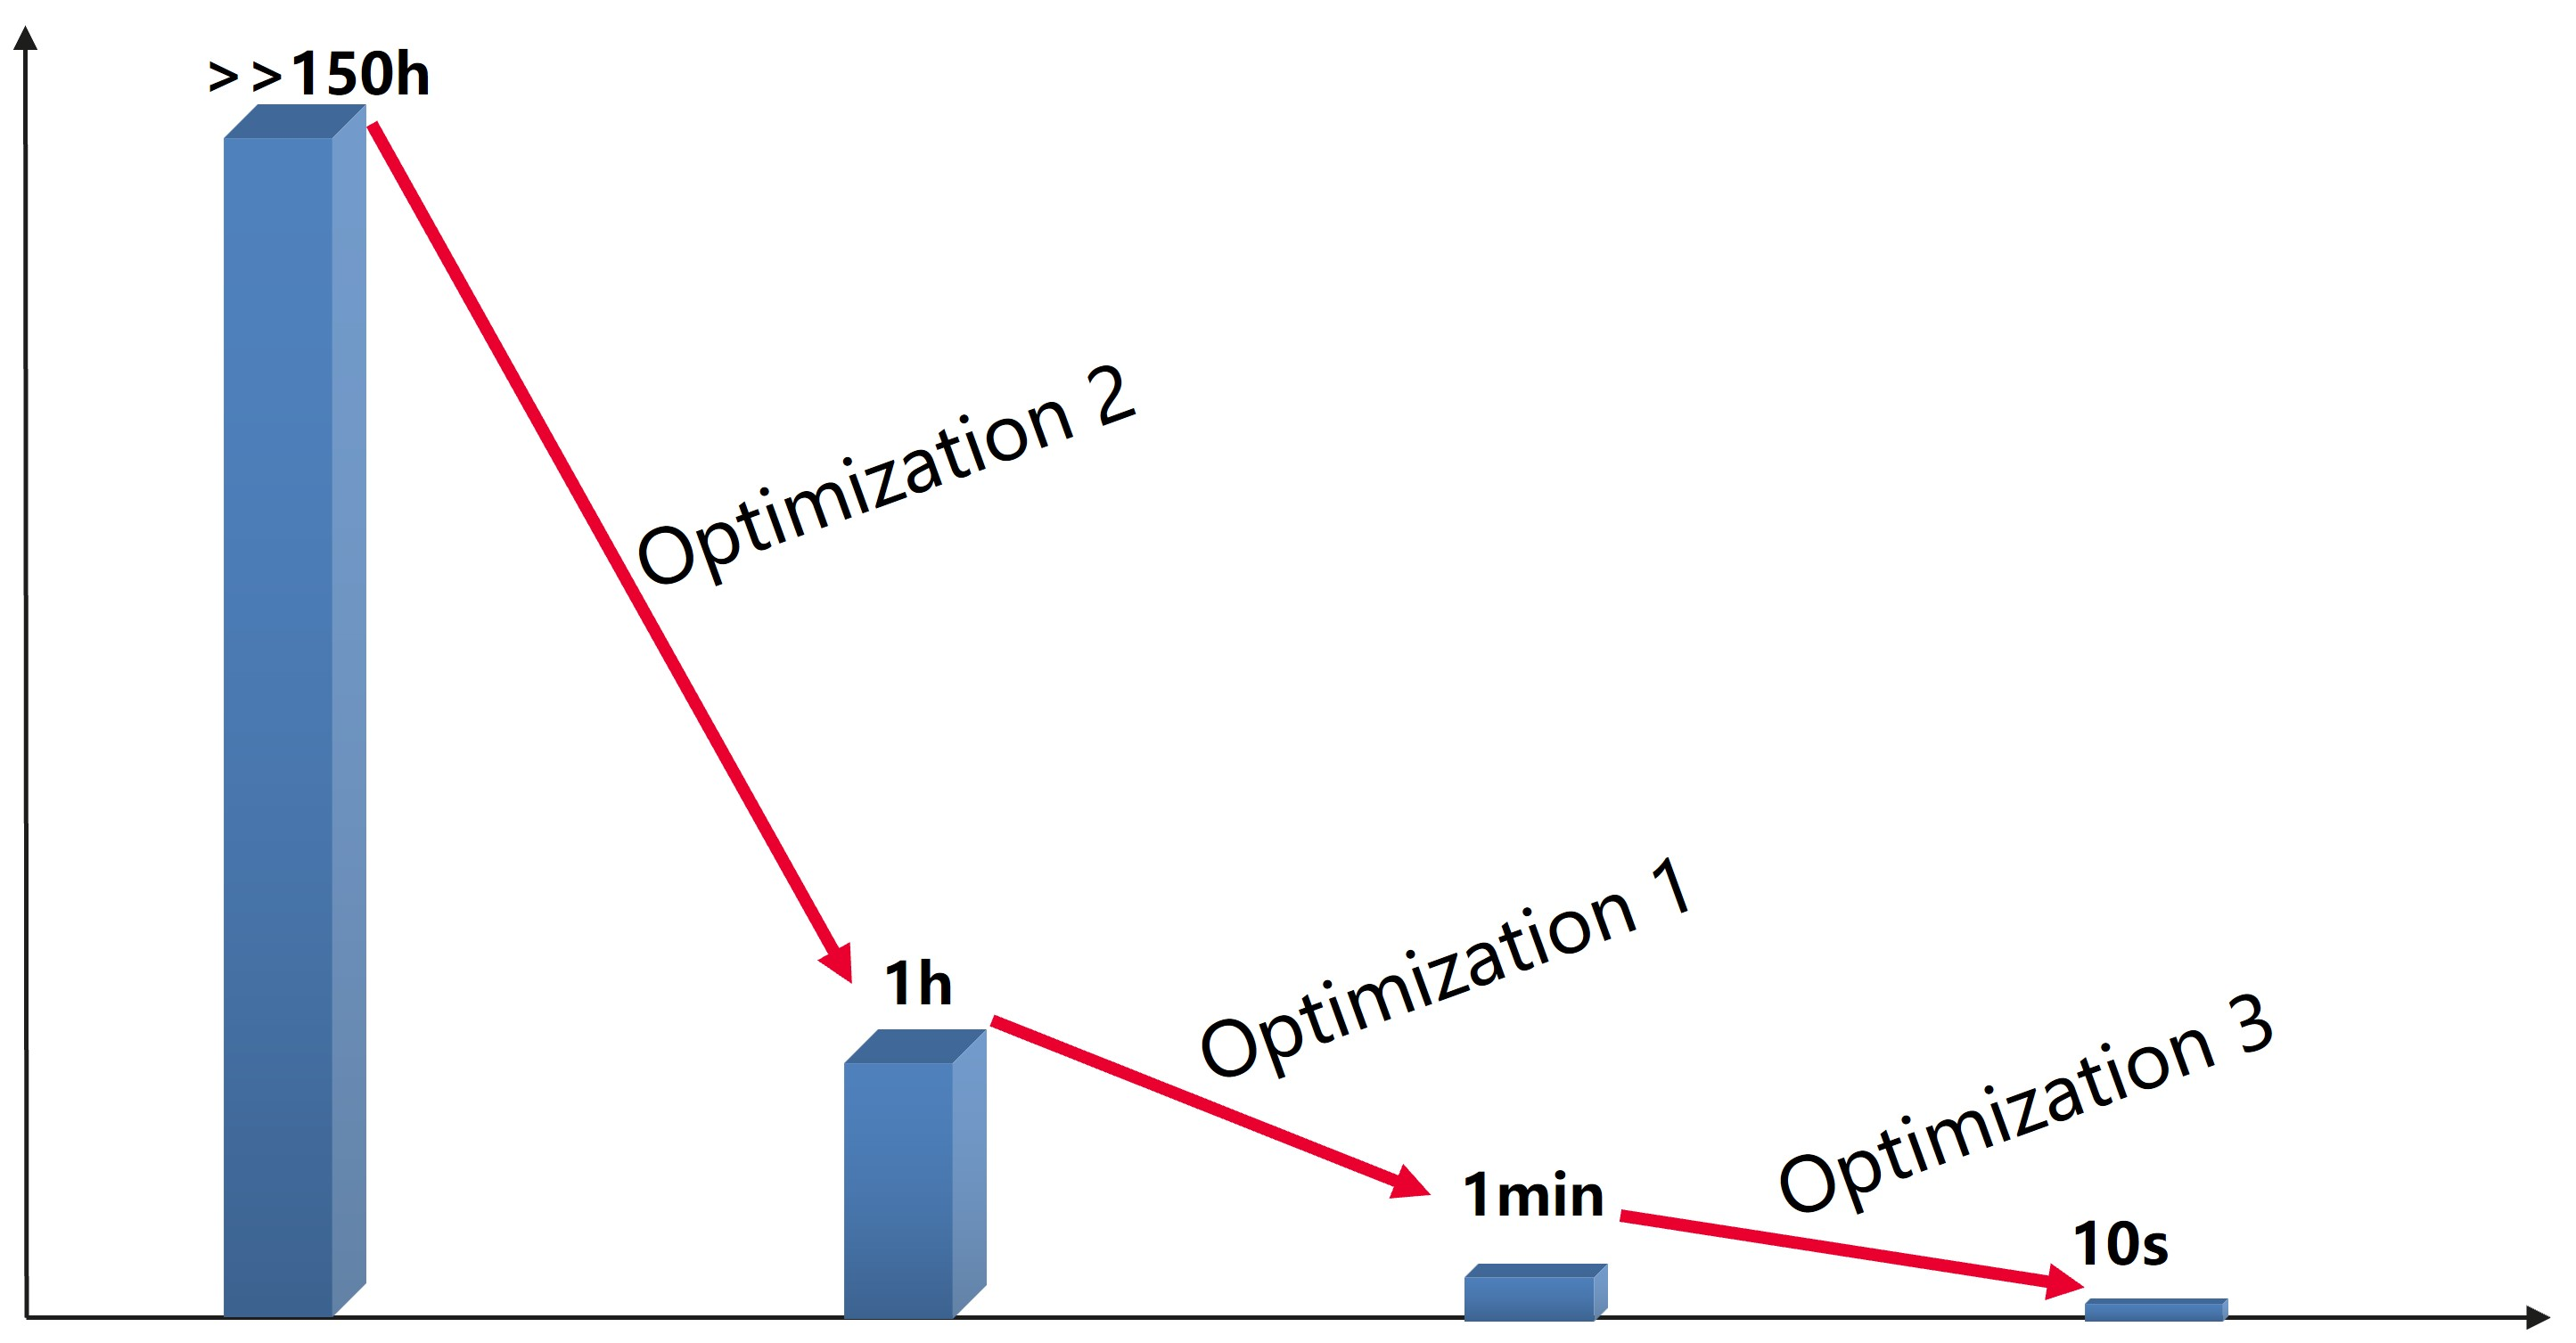
\includegraphics[width = 8cm]{figs/implement/OptEffect.jpg}
	\caption{\small Impact of each optimization on the
 approximate running time of the scheduling algorithm per time slo}
	\label{fig:OptEffect}
\end{figure} 